\section{Gamification}
\subsection{Overview}
Learning Management Systems (LMS) are often only used as tools to distribute course content in various forms and act as a communication tool between course staff and students. Many LMS do not provide features that actively engage, retain and influence students for a better academic outcome.
Gamification of LMS can achieve this through an interactive and immersive approach by applying game-like mechanics, creating a fun learning experience for students. 
A Gamification feature must also link seamlessly into a wider meta-lms to ensure course content can be easily retrieved, reused and updated to provide a high-quality learning journey for students.

\subsection{Introduction to LMS Gamification}
Gamification of a Learning System is defined as implementing game thinking and game mechanics into core features of the platform to provide a more interactive learning experience for students. Gamification is built on three simple concepts: Objectives, Rewards and Competition. Objectives can be set by platform admins, aligning to specific course learning objectives. 
These objectives provide students with a purpose to remain on the platform and ultimately achieve course learning outcomes. A reward system is a positive reinforcement for students and can be a driving factor for students to stay on the platform. In a well designed gamification experience, competitive interest pushes students to perform better and to gain more knowledge to attain a higher position than others. 
Through these fairly simple concepts, the gamification feature in a learning management system can help students achieve course learning objectives in an immersive and rewarding manner.

\newpage

\subsection{Goal Of Gamification Feature}
The goal of this feature is to form a crucial component in the meta-lms to provide a reusable, customisable and seamless experience for course admins as well as a fun, interactive and immersive learning experience for students using the platform. This feature aims to implement the 3 gamification concepts of Objectives, Rewards and Competition. 
The gamification feature will be structured into levels with Core Knowledge modules providing clear objectives for students, Challenge modules providing practical hands on practice that when combined with the reward system create a competitive environment for students. These modules will provide a level of customisation based on wider lms permissions to academics. Academics can customise the questions and question types in each module, set the correct answers as well as set the achievement / rewards that students will earn on completion.
The types of games in scope for development will be multiple-choice style (Timed and Untimed) games, True / False games and coding questions (Assessed on test suite). The feature will also enable academics to customise the levels and select the games they like to be included in their course run. The Gamification feature will be integrated into the larger meta-lms where the data is stored.

\begin{itemize}
    \item High Levels of Engagement and Retention on Platform
    \item Present content with a fun and immersive approach
    \item Better retention and improved proficiency through practice
    \item Challenge and stimulate creativity
    \item Trigger change in thinking
    \item Influence positive behavioral change
\end{itemize}

\newpage


\subsection{Functional Requirements}
Since the backend for the Meta LMS is being built out independently to the individual features, the following contains a description of the ideal backend design for the forum component.

\subsubsection{Learning Structure}
\begin{figure}[h!]
    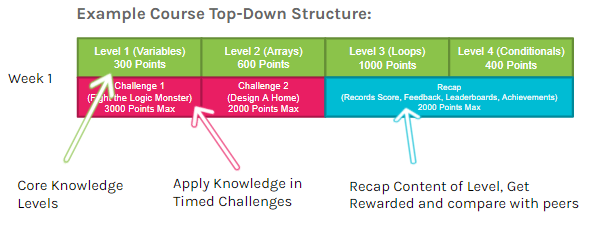
\includegraphics[scale=1.5]{gamification-structure.png}
    \centering
    \caption{Learning Level Structure}
\end{figure}

The above outlines the learning structure for the gamification feature. This includes Core Knowledge modules that can be set as objectives for the week. Academics can customise the content and the number of these core knowledge modules which should be broken down by topics (E.g. Variables, Arrays, Loops). The Challenge module allows academics to create challenging practical exercises for students to apply their knowledge learnt in core knowledge modules. Academics can set the rewards and achievements that students will earn in each of the different modules. These rewards will allow the system to automatically produce leaderboards and in game prompts to drive a competitive environment.

\subsubsection{Core Knowledge Modules}
Core Knowledge modules will have functionality to add video content, content from webpage as well as pdf content. After these content, several game types can be added (MCQ, True/False, Coding Questions) to test the knowledge students just learnt. Core Knowledge modules can be set as prerequisite for challenges and allow the students to earn reward points as well. Core Knowledge modules will be used to introduce specific topics through short videos followed by questions to test the newly gained knowledge. 

\subsubsection{Challenge Modules}
Challenges are more challenging timed games where students need to apply the core knowledge in various ways to earn points. This reinforces and simulates a review of the core knowledge. Challenges are timed levels with a higher difficulty level but provide students with the most rewards based on their performance (Time Taken and Accuracy Of Answers).

\subsubsection{Reward System}
In Core Knowledge and Challenge modules, students can earn points based on their accuracy in answering questions under time pressure. The number of points earned per activity can be customised by course admin. These points will be recorded for modules, weeks and all time to generate leaderboards. Based on points earned and certain criteria, the platform can issue an achievement that is unique and only be earned once per course. These achievements can be customised by the course admin. Students will be able to use the points earned to redeem items that will help them earn more points. Some examples: x2 points for 1 hour. 

\subsubsection{Game Types}
Game Types in scope are Timed or Untimed multiple choice questions, True / False questions as well as coding questions (through integrated text editor). The game type structures pull data from the meta-lms database that are related to their specific data structure. Course admins will be able to create, customise and choose reward parameters for each game type. This feature will be implemented to be easily modified to include more game types in the future.

\subsubsection{Student Frontend Requirements}
\begin{enumerate}
    \item As a Student, I need to be able to access the gamification feature to navigate and complete modules for my course. (Permissions)
    \item As a Student, I need to be able to complete Core Knowledge Modules. (Course)
    \item As a Student, I need to be able to complete Challenge Modules. (Course)
    \item As a Student, I need to be able to see a recap of my progress in level. (Course)
    \item As a Student, I need to be able to view all my enrolled courses and access weekly activities. (Course)
    \item As a Student, I need to be able to monitor my progress compared to other students. (Course)
    \item As a Student, I need to be able to see my achievements and reward points. (Rewards)
    \item As a Student, I need to be able to see my leaderboard rankings compared to my peers. (Rewards)
\end{enumerate}

\subsubsection{Academic Frontend Requirements}
\begin{enumerate}
    \item As an Academic, I need to be able to access the gamification feature to navigate, customise courses and set permissions for students. (Permissions)
    \item As an Academic, I need to be able to create a new course run either new or clone from previous course. (Course Management)
    \item As an Academic, I need to be able to customise content and number of questions for Core Knowledge Modules and Challenge Modules. (Course Management)
    \item As an Academic, I need to be able to create new timed or untimed questions of types (MCQ, True / False, Coding). (Course Management)
    \item As an Academic, I need to be able to monitor the leaderboards for the course and monitor course level statistics. (Course Management)
    \item As an Academic, I need to be able to customise the rewards awarded to students on completion of questions in modules. (Rewards Management)
\end{enumerate}

\newpage

\subsubsection{Backend Requirements}
Gamification Feature will require some backend connections to the meta-lms to setup for integration of permissions, content and results.
This feature will also need backend functions that will enable setup and customisation of courses, modules and student profiles.

\begin{enumerate}
    \item Retrieve a list of students enrolled in course from meta-lms
    \item Retrieve a list of all or courses in meta-lms
    \item Retrieve a list of all or course games
    \item Retrieve a list of levels in course
    \item Retrieve individual post details for post page (including comments and responses)
    \item Retrieve permissions for user
    \item Store course
    \item Store level
    \item Store game
    \item Update game
    \item Update level
    \item Update course
    \item Update user rewards
    \item Update permissions for user
\end{enumerate}

\subsection{Software Development Approach}
In this new gamification feature for the meta-lms, we will be using React as our frontend architecture. It is the most modern and widely used framework that will ensure the longevity of this feature.
While React is used as a frontend framework, node js is used as a middle layer for data manipulation and api creation. Node js is a simple framework based on js that allows for quick development of REST APIs that are hosted on the web server. The data manipulation layer will interact with the PostgreSQL backend which will hold all the data for the meta-lms.
Gamification feature will have its own suite of REST APIs developed that are specific to implementation of the 3 concepts.

\begin{enumerate}
    \item Data Structure for Gamification will first be set up in the PostgreSQL. These include the SQL tables required and a UML diagram to outline how each table will interact with one another.
    \item REST APIs created to facilitate interactions between frontend and backend.
    \item Frontend Development
    \item Testing of Gamification Feature
    \item Integration to meta-lms
\end{enumerate}

\subsection{Evaluation}
Before implementation, we need to understand our users (Academics and Students). In Term 2, we will provide several students and academics with a questionnaire surveying knowledge about gamification as well as popular features and use cases in a gamified LMS. Using the survey, we can test and refine our initial user stories to ensure we meet the end user’s needs.

To evaluate the quality of the implementation, the gamification feature must be integrated into the wider meta-lms and pass various feature specific automated tests as well as meta-lms automated tests. These tests will ensure that the feature is performing to its specifications and that this remains through when operating it as an integrated feature in the meta-lms.

On completion of a working prototype of the meta-lms gamification feature, we will conduct user testing that will help to refine and iron out issues with the platform. The user testing will include hands-on interaction with the prototype running through various use cases on the gamified lms. Upon completion we will utilise the feedback from user testing to refine the platform. Success of the thesis will determine completion of the gamified LMS feature with positive user feedback for the platform.

\newpage

\subsection{Project Timeline}
Below is a rough guideline of some milestones that should be met throughout the year in order to complete this feature on time.

\begin{figure}[h!]
    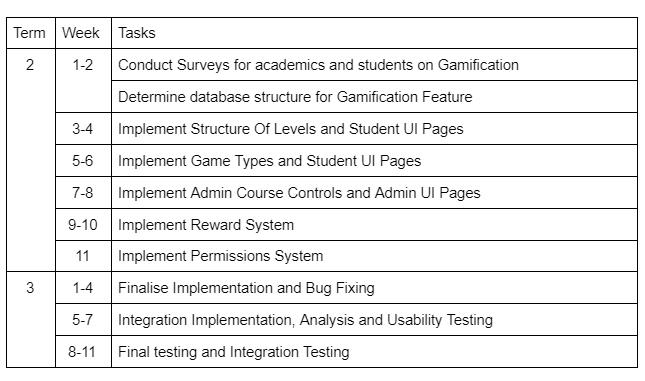
\includegraphics[scale=1.5]{gamification-plan.png}
    \centering
    \caption{Term 2 and 3 Project Implementation Timeline}
\end{figure}

\newpage